\subsection{\label{sub:\projectname-sel} \textsf{sel}}

\paragraph{Símbol}

\begin{center} \bsfsymbol{sel} \end{center}

\paragraph{Entrades i sortides}

\begin{where}
\item[\nodenamebit{sigRes}] Signe del resultat actual
\item[\nodenamerange{res}{7}{0}] Mòdul del resultat actual (BCD)
\item[\nodenamebit{show}] Senyal que s'activa si s'ha de mostrar el resultat
\item[\nodenamebit{sigSel}] Signe a visualitzar als displays del resultat
\item[\nodenamerange{sel}{7}{0}] Mòdul a visualitzar als displays del resultat (BCD$^\dagger$)
\end{where}

\paragraph{Funció}

Controla la sortida del bloc multiplicador, que posteriorment serà convertida a set-segments
i es mostrarà als displays del resultat.

Si $show$ és actiu, la sortida $sel$ és directament l'entrada $res$, i el mateix amb $sigSel$ i $sigRes$.
En cas contrari, la sortida són xifres BCD invàlides per tal d'apagar els displays que mostren el resultat,
i signe positiu per al mateix propòsit.

\paragraph{Inespecificacions}

Cap.

\paragraph{Notes}

El funcionament d'aquest bloc es basa en que els conversors a set-segments
apaguen els displays per a una xifra BCD invàlida, i per a signe positiu.
Això és el cas per a \textsf{BCD7seg} i \textsf{CA2\_SIG\_SS}.

\paragraph{Implementació}

\vhdlisting{sel}



% FIXME

\paragraph{Simulació}

\begin{contendfig}
  \begin{center}
    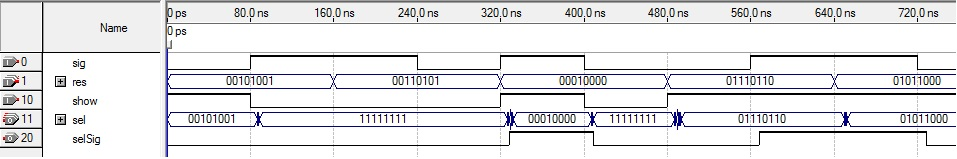
\includegraphics[scale=0.55]{../\projectname/assets/vwf/sel.jpg}
  \end{center}
  \caption{\label{fig:sim-\projectname-sel} Simulació per al bloc \textsf{sel}}
\end{contendfig}

La simulació del bloc es pot veure a la figura~\ref{fig:sim-\projectname-sel} (pàgina~\pageref{fig:sim-\projectname-sel}).

% FIXME

\vspace{1cm}
